\documentclass[conference]{IEEEtran}
\IEEEoverridecommandlockouts
% The preceding line is only needed to identify funding in the first footnote. If that is unneeded, please comment it out.
\usepackage{ctex}
\usepackage{cite}
\usepackage{amsmath,amssymb,amsfonts}
\usepackage{algorithmic}
\usepackage{graphicx}
\usepackage{textcomp}
\usepackage{xcolor}
\def\BibTeX{{\rm B\kern-.05em{\sc i\kern-.025em b}\kern-.08em
    T\kern-.1667em\lower.7ex\hbox{E}\kern-.125emX}}
\begin{document}


% \title{文章标题}

% \author{
% \IEEEauthorblockN{张三}
% \and
% \IEEEauthorblockN{李四}
% }

% \maketitle

\input{title.tex}

\begin{abstract}
论文摘要是对文章内容不加诠释和评论的简单陈述。一般控制在 200 字左右,建议在论文全部完成后再动手写摘要。
\end{abstract}


\section{引言}

本项目旨在解决Unity多人在线对战游戏开发的问题,联机系统为C/S模式,使用Socket技术自主开发。该游戏是一个基于物理的足球游戏,打开游戏并设定好端口号后即开启了服务端,其他人则只需输入专用服务器的IP地址和端口号便可加入游戏,即使是中途加入当前场上的状态也会同步过来;每位连接到服务器的玩家都会在一定规则下被分配到队伍,将球踢入其他队伍球门会加分,踢入自己队伍球门会扣分;玩家在游戏中有着丰富多样的策略,可以通过身体来带球,可以用四个角上的能量棒去“踢”球,还可以通过旋转能量棒改变球的走向,甚至借助蓄力来发动必杀技,一转局势;因为完全基于物理,玩家的移动等操作皆是通过施加力来实现的,不同物体的物理材质也有差异,如运用得当,可完成多次反弹进门等高难度操作;小地图、碰撞效果、蓄力显示等将给予玩家非常直观的反馈。

“独乐乐不如众乐乐”,多人游戏与单人游戏的快乐程度是在不同层次上的,不管是棋牌类的斗地主、麻将,还是竞技类的足球、篮球,亦或是流行的电子游戏《魔兽争霸》《英雄联盟》都为玩家们带来了单人时无法获得的快乐,许多人还会去观看其他人直播游玩多人游戏,从中获得欢愉。多人游戏也极大拓宽了一个游戏的丰富度,一个规则设置和维护得当的游戏,玩家可以游玩数年也不会感到厌倦。从开发的角度上,将一款游戏做成联机游戏的难度也与纯本地游戏是不可同日而语的,从建立连接、收发数据包到同步状态,还要考虑延迟、反作弊等各种复杂问题,Unity本身也没有内置合适的联网组件,这些对开发者来说都是一种考验。

我们在开题之初便对常用的Unity联网游戏实现方式进行了调研。首先,Unity内置的Unity Networking(UNet)已经被官方宣布为过时,并将在近两年彻底停止维护,从Unity中移除\cite{UNet过时};官方用于取代UNet的新联网组件——基于ECS架构的Unity NetCode,最新版本刚发布到 0.2.0,只是预览测试用的版本,无法正式投入实际开发;对于第三方的解决方案,Mirror算是基于UNet的改进版,但每个连接仅支持一个客户端;SmartFoxServer知名度低,国内外的文档都比较少;Photon为Client/Client的通信模式,并非我们需要的Client/Server模式\cite{优缺点比较},ET框架是一个组件系统,和我们熟悉的面向对象差异较大。综合考虑各个因素,小组成员决定通过较为底层的Socket直接开发我们希望实现的网络联机系统,相关代码完全透明,参考微软提供的.NET文档,有着高度的自定义性,也不用担心因第三方封装带来的未知bug。

我们从最基础的连接和收发包开始,先建立一个控制台的服务器和Unity中的客户端,接下来将服务器迁移到Unity中,随后再将二者合到一个项目中,共用场景。与此同时,本地也有一个测试场景,用来完成上线前的调试工作。网络部分,我们专注于场景中物体的创建、销毁、同步……玩家角色作为游戏中最重要的部分之一,从基础的移动逐渐丰富到能蓄力、能施展必杀技,有些效果的实现可能会对联网部分提出新的要求,此时便会一边开发网络部分,一边在本地开发效果部分。最后,还有一些用来增加游戏表现力的后期处理和辅助开发的实用代码。


\section{相关工作(飞)}
\subsection{Unity}
Unity是一个跨平台的游戏引擎,可用于创建三维、二维、VR、AR游戏,有着可视化编辑、操作简单、文档全面等优点,易于开发学习,深受大众的喜爱。《城市:天际线》《奥日与黑暗森林》《茶杯头》《人类一败涂地》等知名游戏皆是用Unity开发的。

\subsection{C\# Socket}
套接字是支持TCP/IP协议的网络通信的基本操作单元。可以将套接字看作不同主机间的进程进行双向通信的端点,它构成了单个主机内及整个网络间的编程界面。套接字存在于通信域中,各种进程使用这个相同的域用Internet协议来进行相互之间的通信。\cite{Unity3D网络游戏实战}

\begin{figure}[htbp]
    \centerline{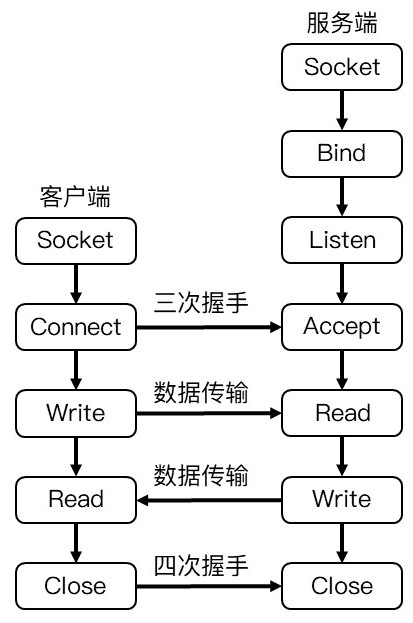
\includegraphics[width=.22\textwidth]{images/Socket通信的基本流程.jpg}}
    \caption{Socket通信的基本流程}
    \label{fig:figure1}
\end{figure}


\subsection{Addressable Asset System}
Addressable Asset System提供了一种按地址加载Assets的简单方式,相比Resources和Asset Bundle更加方便与灵活,能够进行自动化仓储管理和内存管理,只需要一个地址便可以从任意地方加载,默认的所有操作都是异步操作,可以添加事件监听。

\subsection{Post Processing}



相关工作小节主要写和本文主题密切相关的技术/知识点,方便第三节的阐述。

比如本文需要做一个图像识别算法,那本节可以介绍常见的图像识别算法;或者本文主要基于方法 A 进行改进,本节可以对方法 A 进行介绍。

\subsection{子小节}

一般从第二节开始,会出现子小节,请按照逻辑合理组织论文。

\section{实践过程}

\subsection{Socket通信与数据包}
\subsubsection{连接}
\subsubsection{收发包}

\subsection{场景物体}
\subsubsection{资源管理}
\subsubsection{创建}
\subsubsection{销毁}
\subsubsection{同步}
\subsubsection{物理}


\subsection{玩家角色}
\subsubsection{移动}
\subsubsection{蓄力}
\subsubsection{必杀技}
\subsubsection{动画}
\subsubsection{队伍、球门和得分}


\subsection{游戏效果}
\subsubsection{玩家名字}
\subsubsection{小地图}
\subsubsection{后期处理}
\subsubsection{shader(天)}


\subsection{实用代码}
\subsubsection{单例爷爷}
\subsubsection{线程管理}


% \subsection{游戏逻辑}
% \subsubsection{物体基类}
% \subsubsection{资源管理}
% \subsubsection{物体创建}
% \subsubsection{玩家角色}
% \subsubsection{特性}

% \subsection{服务器}
% \subsubsection{物理}
% \subsubsection{控制玩家角色}
% \subsubsection{大招}
% \subsubsection{状态同步}

% \subsection{客户端}
% \subsubsection{相机追踪}
% \subsubsection{玩家输入}
% \subsubsection{后期特效}
% \subsubsection{蓄力}





本节需要详细介绍本文提出/设计的方法。

公式示例:
\begin{equation}
a+b=\gamma\label{eq:demo}
\end{equation}
式~(\ref{eq:demo})是一个演示用的公式。

表格示例。
\begin{table}[htbp]
\caption{表格}
\begin{center}
\begin{tabular}{|c|c|c|c|}
\hline
\textbf{Table}&\multicolumn{3}{|c|}{\textbf{Table Column Head}} \\
\cline{2-4} 
\textbf{Head} & \textbf{\textit{Table column subhead}}& \textbf{\textit{Subhead}}& \textbf{\textit{Subhead}} \\
\hline
copy& More table copy$^{\mathrm{a}}$& &  \\
\hline
\multicolumn{4}{l}{$^{\mathrm{a}}$Sample of a Table footnote.}
\end{tabular}
\label{tbl:test}
\end{center}
\end{table}
表格的代码可以实现在 http://www.tablesgenerator.com/ 上设计好,然后复制过来。表格~\ref{tbl:test}是一个示例。

图片的示例:
\begin{figure}[htbp]
\centerline{
\includegraphics{images/fig1.png}}
\caption{Example of a figure caption.}
\label{fig:figure-1}
\end{figure}
图~\ref{fig:figure1}是一个点。在表格和图中使用 label 可以指定标签,便于后续使用 ref 命令引用。

%参考文献\cite{IEEEexample:softonline,IEEEexample:tamethebeast,IEEEexample:standard}需要先将参考文献的信息写入一个 bib 文件,然后在最后一小节中使用 bibliography 命令指定 bib 文件\cite{IEEEexample:urlsty},具体参见tex源文件。

正文中通过使用 cite 命令引用参考文献。


\section{实验结果(飞)}
本节题目可以自拟。

主要负责成果展示。


\section{结论}
对整个工作做一个总结,得出结论,并展望未来。
提升游戏性,性能优化(搞一个打开后就是6960的,没有图形界面的,没准服务器就能跑动了)


% \section*{References}

\bibliography{myCite}  
\bibliographystyle{IEEEtran}

\end{document}
